\section{NXT Application Design}
The application on the NXT brick should be responsible for aiming and firing the projectile at the target detected by the Kinect. This requires it to be able to convert the information it receives from the Kinect to usable data, predict where the target will be once positioning is done and position the cannon so that it hits the target when it fires. To ensure that the aiming is precise, a reset is required to have the cannon in the same position every time aiming is necessary. This process is illustrated below:

\begin{figure}[hbtp]
	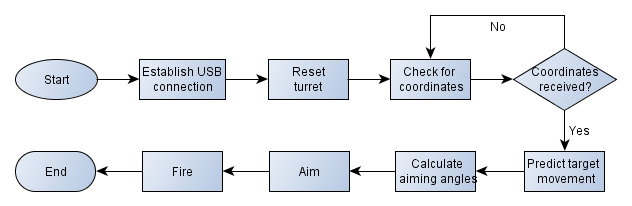
\includegraphics[scale=0.5]{img/nxtdesign.png}
	\caption{Process flow of NXT application}
	\label{nxtdesign}
\end{figure}

As shown, the application should first establish the USB connection to the Kinect via a computer, then reset position of the cannon and wait for the Kinect to supply coordinates. When the coordinates are received, the NXT should calculate where the target will be when the cannon is ready to fire, move the turret accordingly and fire.

This can be broken down into tasks for the NXT program, closely corresponding to the processes in \autoref{nxtdesign}:
\begin{itemize}
	\item Establish USB connection
	\item Reset turret position
	\item Poll for coordinates
	\item When coordinates are received, predict target movement and convert to degrees for the horizontal and vertical motors.
	\item Position horizontally
	\item Position vertically
	\item Fire cannon
\end{itemize}

It would be beneficial to have the same task establish connection to the Kinect and poll for coordinates, and have another task perform both the horizontal and vertical aim, for simplicity.

The conversion from Kinect coordinates to degrees for the motors should incorporate the mathematical equations from \autoref{maththeory} to compensate for gravity.